\documentclass[12pt]{article}
\usepackage{amsmath}
\usepackage{bm}
\usepackage{graphicx}
\usepackage{geometry}
\usepackage{indentfirst}
\usepackage{amsfonts}
\geometry{legalpaper, portrait, margin=0.5in}
\usepackage{color}   %May be necessary if you want to color links
\usepackage{hyperref}
\hypersetup{
    colorlinks=true, %set true if you want colored links
    linktoc=all,     %set to all if you want both sections and subsections linked
    linkcolor=black,  %choose some color if you want links to stand out
}
\usepackage[siunitx]{circuitikz}
\usetikzlibrary{patterns}
\usetikzlibrary{decorations.markings}
\graphicspath{ {./images/} }
\usepackage{enumitem}
\begin{document}
\newcommand*\dif{\mathop{}\!\mathrm{d}}

\setlist[enumerate]{noitemsep, topsep=0pt, leftmargin=2.5\parindent}
\setlist[itemize]{noitemsep, topsep=0pt, leftmargin=2.5\parindent}

\newenvironment{subitemize}
{ \begin{itemize}[leftmargin=\parindent] }
{ \end{itemize} }

\newenvironment{subenumerate}
{ \begin{enumerate}[leftmargin=\parindent] }
{ \end{enumerate} }

\newenvironment{nopagebr}
  {\par\nobreak\vfil\penalty0\vfilneg
   \vtop\bgroup}
  {\par\xdef\tpd{\the\prevdepth}\egroup
   \prevdepth=\tpd}

\tableofcontents

\addcontentsline{toc}{section}{Table of contents}
 
\pagebreak

\section{Modeling}

\subsection{Splines}

\subsubsection{Cubic Hermite Interpolation}

Each point is defined by its position $h_n$ and slope $h_{m + n}$, $m$ being the number of control points. To simplify calculations,
it is assumed that $t_0 = 0$ and $t_1 = 1$.

The goal is to convert from a monomial basis
\begin{align*}
    \phi_0(t) &= 1\\
    \phi_1(t) &= t\\
    \phi_2(t) &= t^2\\
    \phi_3(t) &= t^3
\end{align*}

to a hermite basis
\begin{align*}
    H_0(t) &= 2t^3 - 3t^2 + 1\\
    H_1(t) &= -2t^3 + 3t^2\\
    H_2(t) &= t^3 - 2t^2 + t\\
    H_3(t) &= t^3 - t^2
\end{align*}

so that instead of having to manipulate polynomial coefficients
\[ f(t) = a\phi_3(t) + b\phi_2(t) + c\phi_1(t) + d\phi_0(t) \]

an easier point slope method can be used:
\[ f(t) = h_0H_0(t) + h_1H_1(t) + h_2H_2(t) + h_3H_3(t) \]

\includegraphics[scale=.5]{images/cubic-hermite-interpolation.png}
\begin{align*}
    h_0 &= P(0) = d\\
    h_1 &= P(1) = a + b + c + d\\
    h_2 &= P'(0) = c\\
    h_3 &= P'(1) = 3a + 2b + c
\end{align*}

Unknowns in this equation are $a$, $b$, $c$, and $d$, so a matrix can be used
to solve the systems of equations:
\[
    \begin{pmatrix}
        0 & 0 & 0 & 1\\
        1 & 1 & 1 & 1\\
        0 & 0 & 1 & 0\\
        3 & 2 & 1 & 0
    \end{pmatrix}
    \begin{pmatrix}
        a\\
        b\\
        c\\
        d
    \end{pmatrix}
    =
    \begin{pmatrix}
        h_0\\
        h_1\\
        h_2\\
        h_3
    \end{pmatrix}
\]

$a$, $b$, $c$, and $d$ can be obtained from $h$ values by inverting the matrix:
\[
    \begin{pmatrix}
        0 & 0 & 0 & 1\\
        1 & 1 & 1 & 1\\
        0 & 0 & 1 & 0\\
        3 & 2 & 1 & 0
    \end{pmatrix}^{-1}
    \begin{pmatrix}
        h_0\\
        h_1\\
        h_2\\
        h_3
    \end{pmatrix}
    =
    \begin{pmatrix}
        a\\
        b\\
        c\\
        d
    \end{pmatrix}
\]

From these solved $h$ values, $P(t)$ can now be converted to a form that is
easier for a user to manipulate, in terms of $h$ values:
\begin{align*}
    P(t) =& \ at^3 + bt^2 + ct + d\\
    =& \ (2h_0 - 2h_1 + h_2 + h_3)t^3\\
        &+ (-3h_0 + 3h_1 - 2h_2 - h_3)t^2\\
        &+ h_2t + h_0\\
    =& \ h_0(2t^3 - 3t^2 + 1) + h_1(-2t^3 + 3t^2) +\\
       & \ h_2(t^3 - 2t^2 + t) + h_3(t^3 - t^2)
\end{align*}

Each equation in $P(t) = h_0(2t^3 - 3t^2 + 1) +
h_1(-2t^3 + 3t^2) + h_2(t^3 - 2t^2 + t) + h_3(t^3 - t^2)$ that is multiplied
by an $h$ value is called a cubic hermite.

\subsubsection{More than 1D}

A parametric curve described by $\vec \gamma(t) = (\gamma_0(t),
\gamma_1(t))$ can be converted into hermite basis like this:

\includegraphics[scale=.5]{images/parametric-hermite.png}

where cubic hermite interpolation can be done for both dimensions.

\subsubsection{Cubic blossom}

The cubic blossom of a function $\vec f(t)$ is $\vec F(t_1,t_2,t_3)$.

Cubic blossoms have three properties:
\begin{enumerate}
    \item Symmetric
        \begin{subitemize}
            \item $\vec F(t_1,t_2,t_3) = \vec F(t_1,t_3,t_2) = \vec F(t_3,t_1,t_2) \cdots$
        \end{subitemize}
    \item Affine
        \begin{subitemize}
            \item $\vec F(\alpha u + (1-\alpha)v,t_2,t_3) = \alpha \vec F(u,t_2,t_3) + 
                 (1-\alpha)\vec F(v,t_2,t_3)$
            \item If only one of $\vec F$'s arguments $t_c = \alpha u +
                (1-\alpha)v$ is changing between different points on $\vec F$,
                then any value $\vec F(t_c,t_2,t_3)$ in between $\vec F(u,t_2,t_3)$ and
                $\vec F(v,t_2,t_3)$ is scaled equivalently with $\alpha$ like
                $t_c$ is scaled between $u$ and $v$.
                
        \end{subitemize}
    \item Diagonal
        \begin{subitemize}
            \item $\vec f(t) = \vec F(t,t,t)$
        \end{subitemize}
\end{enumerate}

Blossoming examples
\begin{itemize}
    \item $\vec f(t) = t^3 \mapsto \vec F(t_1,t_2,t_3) = t_1t_2t_3$
    \item $\vec f(t) = t^2 \mapsto \vec F(t_1,t_2,t_3) = (t_1t_2 + 
            t_1t_3 + t_2t_3)/3$
    \item $\vec f(t) = t \mapsto \vec F(t_1,t_2,t_3) = (t_1 + t_2
            + t_3)/3$
    \item $\vec f(t) = 1 \mapsto \vec F(t_1,t_2,t_3) = 1$
    \item $\vec f(t) = 3t^3 - t + 1 = 3(t_1t_2t_3) - (t_1 + t_2
            + t_3)/3 + 1$
\end{itemize}

Cubic curves can be blossomed by blossoming each coordinate function
separately, which will give a function that maps 3 $t$ variables to
two dimensions $x$ and $y$: $\vec F(t_1,t_2,t_3): \mathbb R^3
\mapsto \mathbb R^2$. A cubic curve can be obtained from a blossom
by specifying four points $\vec F(0,0,0),\vec F(0,0,1),\vec F(0,1,1)
,\vec F(1,1,1)$ (which form a cubic control polygon) and subdividing
the surface given by the selected points (known as the De Castelijau's Algorithm).
Only these four points are required because of the symmetry property of a blossom.

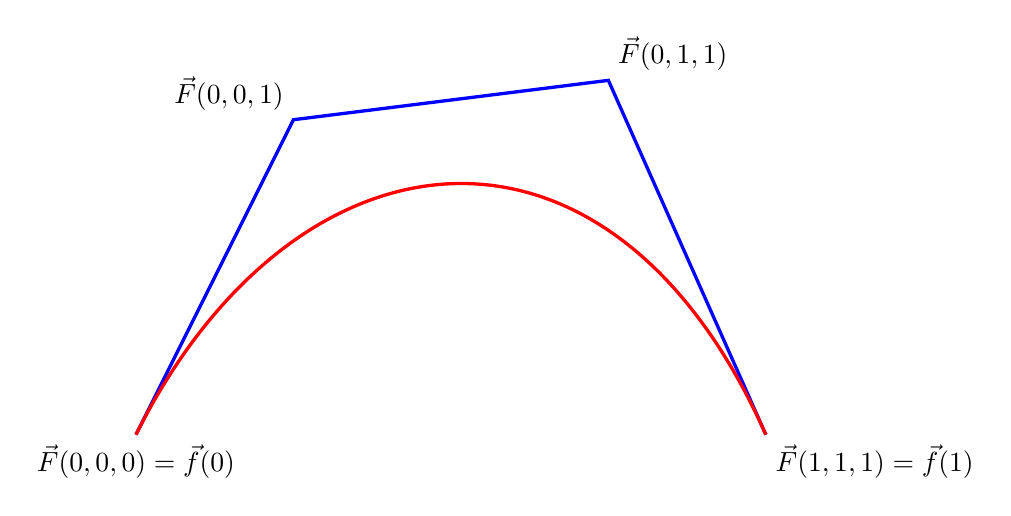
\begin{tikzpicture}
    \draw[color=blue, very thick] (0,0) -- (2,4)
        -- (6,4.5) -- (8,0);
    \draw[color=red, very thick] (0,0) .. controls (2,4) and (6, 4.5) .. (8,0);
    \node[anchor=north] at (0,0) {$\vec F(0,0,0) = \vec f(0)$};
    \node[anchor=south east] at (2,4) {$\vec F(0,0,1)$};
    \node[anchor=south west] at (6,4.5) {$\vec F(0,1,1)$};
    \node[anchor=north west] at (8,0) {$\vec F(1,1,1) = \vec f(1)$};
\end{tikzpicture}

Subdividing the polygon:

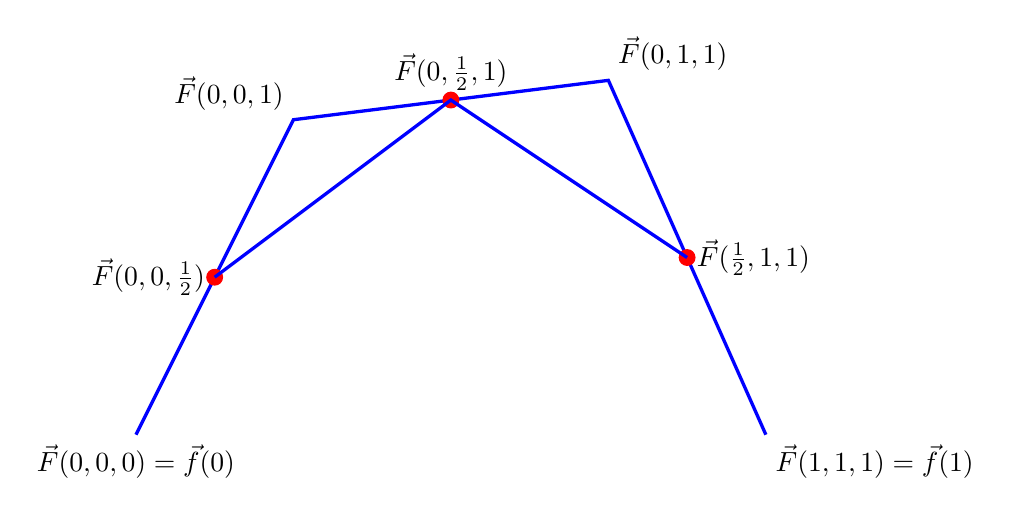
\begin{tikzpicture}
    \draw[color=blue, very thick] (0,0) -- (2,4)
        -- (6,4.5) -- (8,0);
    \node[anchor=north] at (0,0) {$\vec F(0,0,0) = \vec f(0)$};
    \node[anchor=south east] at (2,4) {$\vec F(0,0,1)$};
    \node[anchor=south west] at (6,4.5) {$\vec F(0,1,1)$};
    \node[anchor=north west] at (8,0) {$\vec F(1,1,1) = \vec f(1)$};

    \filldraw[color=red] (1,2) circle (0.1)
            node[color=black, anchor=east] {$\vec F(0,0,\frac 1 2)$};
    \filldraw[color=red] (4,4.25) circle (0.1)
            node[color=black, anchor=south] {$\vec F(0,\frac 1 2,1)$};
    \filldraw[color=red] (7,2.25) circle (0.1)
            node[color=black, anchor=west] {$\vec F(\frac 1 2, 1, 1)$};

    \draw[color=blue, very thick] (1,2) -- (4,4.25) -- (7,2.25);
\end{tikzpicture}

$\vec F$'s arguments at the subdivision points can be determined due to the affine
property of a blossom.

Further subdivision

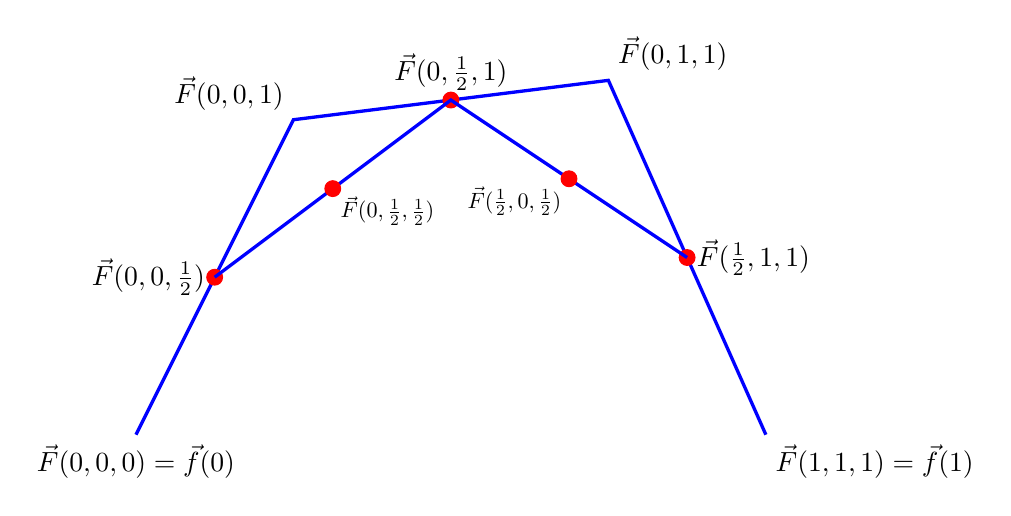
\begin{tikzpicture}
    \draw[color=blue, very thick] (0,0) -- (2,4)
        -- (6,4.5) -- (8,0);
    \node[anchor=north] at (0,0) {$\vec F(0,0,0) = \vec f(0)$};
    \node[anchor=south east] at (2,4) {$\vec F(0,0,1)$};
    \node[anchor=south west] at (6,4.5) {$\vec F(0,1,1)$};
    \node[anchor=north west] at (8,0) {$\vec F(1,1,1) = \vec f(1)$};

    \filldraw[color=red] (1,2) circle (0.1)
            node[color=black, anchor=east] {$\vec F(0,0,\frac 1 2)$};
    \filldraw[color=red] (4,4.25) circle (0.1)
            node[color=black, anchor=south] {$\vec F(0,\frac 1 2,1)$};
    \filldraw[color=red] (7,2.25) circle (0.1)
            node[color=black, anchor=west] {$\vec F(\frac 1 2, 1, 1)$};

    \draw[color=blue, very thick] (1,2) -- (4,4.25) -- (7,2.25);

    \filldraw[color=red] (2.5,3.125) circle (0.1)
            node[color=black, anchor=north west, scale=.8] {$\vec F(0,\frac 1 2,\frac 1 2)$};
    \filldraw[color=red] (5.5,3.25) circle (0.1)
            node[color=black, anchor=north east, scale=.8] {$\vec F(\frac 1 2, 0, \frac 1 2)$};
\end{tikzpicture}

One more subdivision (most recent two subdivision point values omitted
because there's no room left)

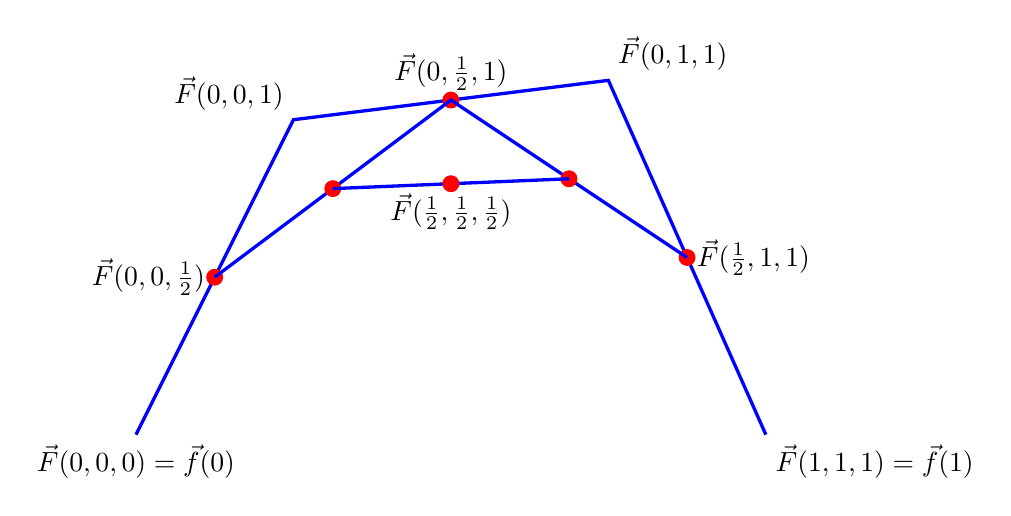
\begin{tikzpicture}
    \draw[color=blue, very thick] (0,0) -- (2,4)
        -- (6,4.5) -- (8,0);
    \node[anchor=north] at (0,0) {$\vec F(0,0,0) = \vec f(0)$};
    \node[anchor=south east] at (2,4) {$\vec F(0,0,1)$};
    \node[anchor=south west] at (6,4.5) {$\vec F(0,1,1)$};
    \node[anchor=north west] at (8,0) {$\vec F(1,1,1) = \vec f(1)$};

    \filldraw[color=red] (1,2) circle (0.1)
            node[color=black, anchor=east] {$\vec F(0,0,\frac 1 2)$};
    \filldraw[color=red] (4,4.25) circle (0.1)
            node[color=black, anchor=south] {$\vec F(0,\frac 1 2,1)$};
    \filldraw[color=red] (7,2.25) circle (0.1)
            node[color=black, anchor=west] {$\vec F(\frac 1 2, 1, 1)$};

    \draw[color=blue, very thick] (1,2) -- (4,4.25) -- (7,2.25);
    \filldraw[color=red] (2.5,3.125) circle (0.1);
    \filldraw[color=red] (5.5,3.25) circle (0.1);
    \draw[color=blue, very thick] (2.5,3.125) -- (5.5,3.25);
    \filldraw[color=red] (4,3.1875) circle (0.1)
            node[color=black, anchor=north] {$\vec F(\frac 1 2, \frac 1 2
            , \frac 1 2)$};
\end{tikzpicture}

The final subdivision point can be shown to equal $\vec f(\frac 1 2)$
because of the diagonal property of blossoms, meaning the $\vec f$ curve
will intersect this third subdivision point:

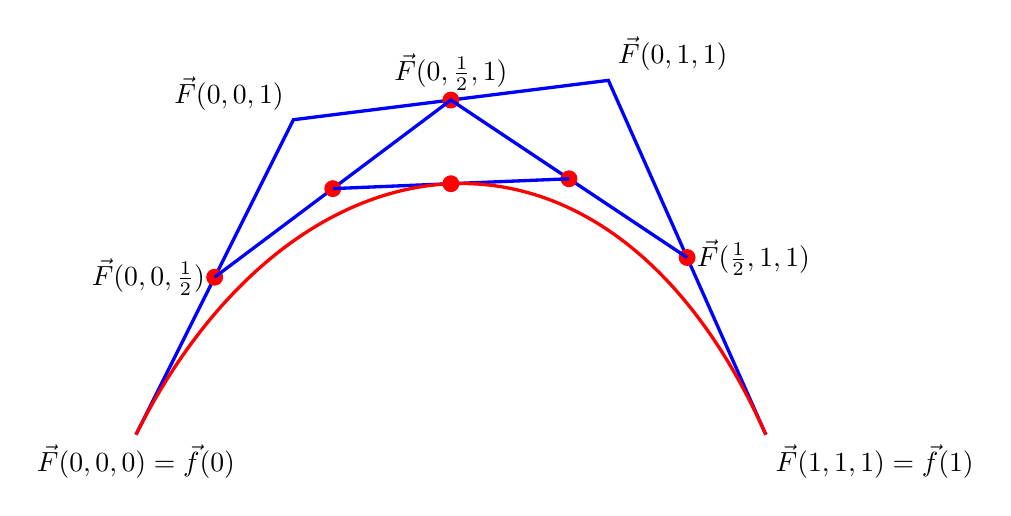
\begin{tikzpicture}
    \draw[color=blue, very thick] (0,0) -- (2,4)
        -- (6,4.5) -- (8,0);
    \node[anchor=north] at (0,0) {$\vec F(0,0,0) = \vec f(0)$};
    \node[anchor=south east] at (2,4) {$\vec F(0,0,1)$};
    \node[anchor=south west] at (6,4.5) {$\vec F(0,1,1)$};
    \node[anchor=north west] at (8,0) {$\vec F(1,1,1) = \vec f(1)$};

    \filldraw[color=red] (1,2) circle (0.1)
            node[color=black, anchor=east] {$\vec F(0,0,\frac 1 2)$};
    \filldraw[color=red] (4,4.25) circle (0.1)
            node[color=black, anchor=south] {$\vec F(0,\frac 1 2,1)$};
    \filldraw[color=red] (7,2.25) circle (0.1)
            node[color=black, anchor=west] {$\vec F(\frac 1 2, 1, 1)$};

    \draw[color=blue, very thick] (1,2) -- (4,4.25) -- (7,2.25);
    \filldraw[color=red] (2.5,3.125) circle (0.1);
    \filldraw[color=red] (5.5,3.25) circle (0.1);
    \draw[color=blue, very thick] (2.5,3.125) -- (5.5,3.25);

    \filldraw[color=red] (4,3.1875) circle (0.1);
    \draw[color=red, very thick] (0,0) .. controls (2,4) and (6, 4.5) .. (8,0);
\end{tikzpicture}

Other values of $\vec f$ can be found with subdividing the cubic control
polygon on different values. For example, to find $\vec f(\frac 1 4)$,
each edge would be divided $\frac 1 4$ of the way along it.

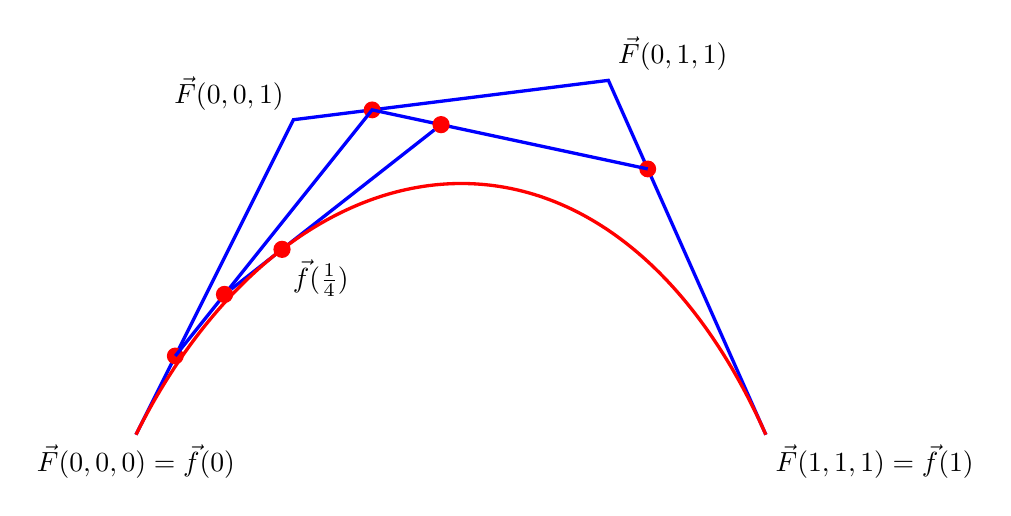
\begin{tikzpicture}
    \draw[color=blue, very thick] (0,0) -- (2,4)
        -- (6,4.5) -- (8,0);
    \node[anchor=north] at (0,0) {$\vec F(0,0,0) = \vec f(0)$};
    \node[anchor=south east] at (2,4) {$\vec F(0,0,1)$};
    \node[anchor=south west] at (6,4.5) {$\vec F(0,1,1)$};
    \node[anchor=north west] at (8,0) {$\vec F(1,1,1) = \vec f(1)$};

    \filldraw[color=red] (.5,1) circle (0.1);
    \filldraw[color=red] (3,4.125) circle (0.1);
    \filldraw[color=red] (6.5,3.375) circle (0.1);

    \draw[color=blue, very thick] (.5,1) -- (3,4.125)
        node[pos=.25,draw=red,fill=red,shape=circle,
        minimum size=5pt,inner sep=0pt] (A) {} -- (6.5,3.375)
        node[pos=.25,draw=red,fill=red,shape=circle,
        minimum size=5pt,inner sep=0pt] (B) {};
    \draw[color=blue, very thick] (A) -- (B)
        node[pos=.25, draw=red,fill=red,shape=circle,
        minimum size=5pt,inner sep=0pt] {} node[pos=.25,anchor=north west,
        color=black] {$\vec f(\frac 1 4)$};

    \draw[color=red, very thick] (0,0) .. controls (2,4) and (6, 4.5) .. (8,0);
\end{tikzpicture}

\subsubsection{Bernstein polynomials}

Another basis that can represent cubic curves. Bernstein basis is
canonical for Bezier.

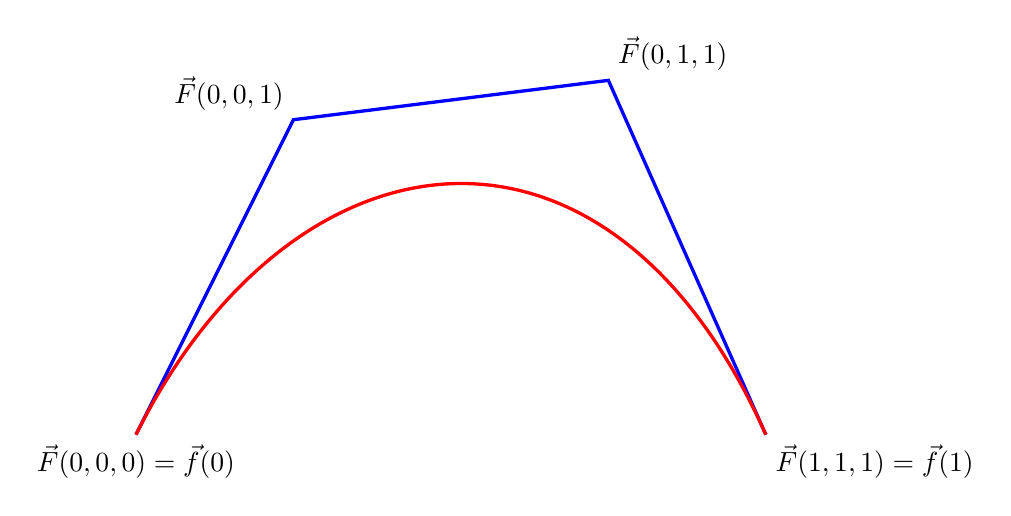
\begin{tikzpicture}
    \draw[color=blue, very thick] (0,0) -- (2,4)
        -- (6,4.5) -- (8,0);
    \draw[color=red, very thick] (0,0) .. controls (2,4) and (6, 4.5) .. (8,0);
    \node[anchor=north] at (0,0) {$\vec F(0,0,0) = \vec f(0)$};
    \node[anchor=south east] at (2,4) {$\vec F(0,0,1)$};
    \node[anchor=south west] at (6,4.5) {$\vec F(0,1,1)$};
    \node[anchor=north west] at (8,0) {$\vec F(1,1,1) = \vec f(1)$};
\end{tikzpicture}

The red curve above can be represented as $\vec f(t) = \vec F(0,0,0)
B_0(t) + \vec F(0,0,1)B_1(t) + \vec F(0,1,1)B_2(t) + F(1,1,1)B_3(t)$, 
knowing
\begin{align*}
    B_0(t) &= (1-t)^3 = 1-3t+3t^2-t^3\\
    B_1(t) &= 3t(1-t)^2 = 3t-6t^2+3t^3\\
    B_2(t) &= 3t^2(1-t) = 3t^2-3t^3\\
    B_3(t) &= t^3
\end{align*}

Changing basis from monomial to Bernstein:
\[
    \begin{pmatrix}
        1 & -3 & 3 & -1\\
        0 & 3 & -6 & 3\\
        0 & 0 & 3 & -3\\
        0 & 0 & 0 & 1
    \end{pmatrix}
    \begin{pmatrix}
        1\\
        t\\
        t^2\\
        t^3
    \end{pmatrix}
    =
    \begin{pmatrix}
        B_0(t)\\
        B_1(t)\\
        B_2(t)\\
        B_3(t)
    \end{pmatrix}
\]

And to change from Bernstein to monomial, the inverse of the matrix
can be used.

\subsubsection{General spline formulation}

$\vec \gamma(t) =$ Geometry $\cdot$ Spline basis $\cdot$ Monomial basis
\begin{itemize}
    \item Geometry contains control point coordinates
    \item Spline basis defines the type of spline (Hermite, Bernstein, etc)
    \item Monomial basis is a column vector $(1,t,t^2,\cdots,t^n)$
\end{itemize}

Example of a spline represented in the Bernstein basis:
\[
    P(t) =
    \begin{pmatrix}
        x(t)\\
        y(t)
    \end{pmatrix}
    =
    \begin{pmatrix}
        x_1 & x_2 & x_3 & x_4\\
        y_1 & y_2 & y_3 & y_4
    \end{pmatrix}
    \begin{pmatrix}
        1 & -3 & 3 & -1\\
        0 & 3 & -6 & 3\\
        0 & 0 & 3 & -3\\
        0 & 0 & 0 & 1
    \end{pmatrix}
    \begin{pmatrix}
        1\\
        t\\
        t^2\\
        t^3
    \end{pmatrix}
\]

\subsubsection{Orders of continuity}

$C^0$ = continuous (seam can be sharp)

$G^1$ = geometric continuity (Tangent vectors align at the seam)

$C^1$ = parametric continuity (Same velocity at the seam)

$C^2$ = curvature continuity (Tangents and tangent derivatives are the same)

\subsubsection{Cubic B-splines}

$\ge$ 4 control points

Chain together splines in fours, popping the back control point off and
pushing the next control point on

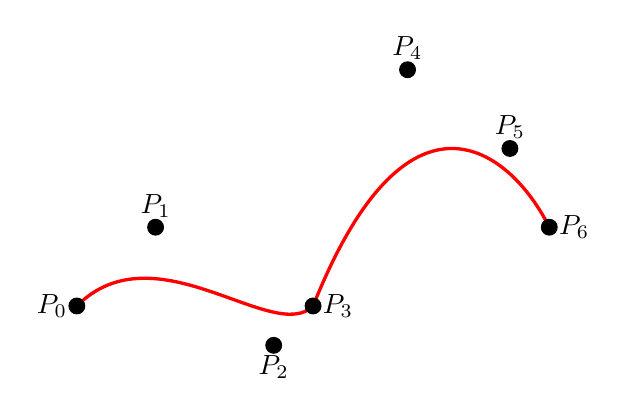
\begin{tikzpicture}
    \draw[color=red,very thick] (0,0) .. controls (1, 1) and (2.5, -.5)
        .. (3, 0) .. controls (4.2,3) and (5.5,2) .. (6,1);
    \filldraw (0,0) circle (.1) node[anchor=east] {$P_0$};
    \filldraw (1,1) circle (.1) node[anchor=south] {$P_1$};
    \filldraw (2.5,-.5) circle (.1) node[anchor=north] {$P_2$};
    \filldraw (3,0) circle (.1) node[anchor=west] {$P_3$};
    \filldraw (4.2,3) circle (.1) node[anchor=south] {$P_4$};
    \filldraw (5.5,2) circle (.1) node[anchor=south] {$P_5$};
    \filldraw (6,1) circle (.1) node[anchor=west] {$P_6$};
\end{tikzpicture}

The full curve is composed of many smaller splines, in which the
$n$th spline is formed by points $P_{n..n+3}$. The benefit of this
method is that it guarantees $C^1$ continuity since every spline shares
three control points with the one that comes before and after it.

The end points won't connect with this method, but repeating endpoints
will fix it.

The basis functions as well as the basis conversion matrix
for cubic b-spline are listed here:
\begin{align*}
    B_1(t) &= \frac 1 6 (1-t)^3\\
    B_2(t) &= \frac 1 6 (3t^3-6t^2+4)\\
    B_3(t) &= \frac 1 6 (-3t^3+3t^2+3t+1)\\
    B_4(t) &= \frac 1 6 t^3
\end{align*}
\[
    B_{B-spline} =
    \frac 1 6
    \begin{pmatrix}
        1 & -3 & 3 & -1\\
        4 & 0 & -6 & 3\\
        1 & 3 & 3 & -3\\
        0 & 0 & 0 & 1
    \end{pmatrix}
\]

\subsubsection{Bezier vs B-spline}

\includegraphics[scale=.5]{images/bezier-vs-bspline.png}

Bezier is derived from Bernstein polynomials, while B-spline uses a
different set of basis functions. Additionally, Bezier will try
to intersect with control points and only guarantees $C^0$ continuity,
while B-spline does not and guarantees $C^1$ continuity.

Converting between bezier and b-spline, given $G$ = geometry,
$B_0$ = current basis matrix, $T(t)$ = monomial basis, and $B_1$ =
the basis matrix to convert to:
\begin{align*}
    \vec \gamma(t) &= G \cdot B_0 \cdot T(t)\\
    &= G \cdot B_0 \cdot B_1^{-1} \cdot B_1 \cdot T(t)\\
    &= (G \cdot B_0 \cdot B_1^{-1}) \cdot B_1 \cdot T(t)
\end{align*}

The new geometry matrix is then represented as $G \cdot B \cdot
B_1^{-1}$, which shows that to convert between bezier and b-spline,
a different set of data is required for the same curve.

\subsection{2D Surfaces}

\subsubsection{Bicubic Bezier surfaces}
\includegraphics[scale=2]{images/surface-example.png}

Given $u$ changes vertically and $v$ changes horizontally,
\begin{align*}
    P(u,v) =& \ (1-u)^3 P_1(v)\\
    &+ 3u(1-u)^2 P_2(v)\\
    &+ 3u^2(1-u) P_3(v)\\
    &+ u^3 P_4(v)
\end{align*}

For any constant $u$ for $0 \le u \le 1$ there is a bezier curve
as a function of $v$ for $0 \le v \le 1$ at that $u$, and vice
versa.

\includegraphics[scale=2]{images/bicubic-bezier-surface.png}
\begin{align*}
    P(u,v) &= \sum_{i=1}^4 B_i(u) P_i(v)\\
    P_i(v) &= \sum_{j=1}^4 B_j(v) P_{i,j}
\end{align*}

Which can be compactly expressed as:
\begin{align*}
    P(u,v) &= \sum_{i=1}^4 B_i(u) \left[ \sum_{j=1}^4 P_{i,j} B_j(v) \right]\\
           &= \sum_{i=1}^4 \sum_{j=1}^4 P_{i,j} B_{i,j}(u,v)
\end{align*}

where $B_{i,j}(u,v) = B_i(u)B_j(v)$.

\subsubsection{Tangents and Normals for patches}

The partial derivatives $\partial P/\partial u$ and
$\partial P/\partial v$ are tangent vectors.

Normal vector is equal to the cross product of the tangent vectors:
\[ \vec N = \frac{\partial P}{\partial u} \times \frac{\partial P}
{\partial v} \]

$\vec N$ is typically not unit, so it needs to be normalized

\subsubsection{Matrix notation for patches}
\[
    P(u,v) =
    \begin{pmatrix}
        B_1(u) & \cdots & B_4(u)
    \end{pmatrix}
    \begin{pmatrix}
        P_{1,1} & \cdots & P_{1,4}\\
        \vdots & \ddots & \vdots\\
        P_{4,1} & \cdots & P_{4,4}
    \end{pmatrix}
    \begin{pmatrix}
        B_1(v)\\
        \vdots\\
        B_4(v)
    \end{pmatrix}
\]

\subsubsection{Implicit surfaces}

$f(x,y,z) = 0$ is on the surface

$f(x,y,z) < 0$ is inside the surface

$f(x,y,z) > 0$ is outside the surface

\subsection{Hierarchical modeling}

\subsubsection{Forward kinematics}

Specifies base position and joint angles. To compute the final position
and orientation of a joint in world coordinates, the motion of all its
ancestor joints must be computed as well.

Given values for joint dof (degree of freedom) $\vec \theta = [\theta_1,\theta_2,
\cdots,\theta_n]^T$, compute the end effector in world space $\vec{\bm e} =
[\bm e_1,\bm e_2,\cdots,\bm e_m]^T$.

$\vec{\bm e} = F(\bm \theta)$

\includegraphics[scale=2]{images/arm.png}

In the diagram above, $P$ in world coordinates can be calculated with
$P_{world} = M_{01}M_{12}M_{23}P_{local}$, or $T(0,6)R(-45)T(5,0)R(50)
T(4,0)R(30)P_{local}P_{local}$, $T$ being a transformation matrix and $R$
being a rotation matrix.

\subsubsection{Inverse kinematics}

Forward kinematics has some issues such as determining what orientation
the arm should be in to interact with other objects, which is what
inverse kinematics aims to solve.

In forward kinematics, $(\bm e_1,\bm e_2) = F(\theta_1,\theta_2,\theta_3)$;
however, in inverse kinematics, $(\theta_1,\theta_2,\theta_3) = G(\bm e_1,
\bm e_2)$.

Inverse kinematics is difficult because sometimes there is no solution / multiple
solutions to a problem. Typically it can't be analytically solved and requires numerical methods.
\begin{itemize}
    \item Jacobian iterative method
    \item Optimization based methods
\end{itemize}

Given position of a point in local coordinates $\bm v_s$ and desired
position in world coordinates $\bm v_w$, find skeleton parameters
$\bm p$.
\[ \bm v_w = S(\bm p)\bm v_s = S(x_h,y_h,z_h,\theta_h,\phi_h,\sigma_h,
\theta_t,\phi_t,\sigma_t,\theta_c,\theta_f,\phi_f) \bm v_s \]

\subsubsection{Jacobian}

$\bm e = F(\bm \theta)$ where $\bm e$ is known and $\bm \theta$
is to be solved for.

The Jacobian is the matrix of partial derivatives
of $\bm F$: $J = \dif F/\dif \bm \theta$

For $\bm F = [\bm F_1,\bm F_2,\cdots,\bm F_m]^T$ and $\bm \theta
= [\theta_1,\theta_2,\cdots,\theta_n]^T$:
\[
    J =
    \begin{bmatrix}
        \frac{\partial \bm F_1}{\partial \theta_1} & \cdots & \frac{\partial F_1}{\partial \theta_n}\\
        \vdots & \ddots & \vdots\\
        \frac{\partial F_m}{\partial \theta_1} & \cdots & \frac{\partial F_m}{\partial \theta_n}
    \end{bmatrix}
\]

\subsection{Skinning}

\subsubsection{SSD}

Skin is made up of vertices, some of which are attached
to a single bone, while others are attached to multiple.

Example

\includegraphics[scale=.4]{images/skinning-vertices.png}

\subsubsection{Vertex weights}

Weight $w_{ij}$ is assigned for each vertex $\bm p_i$ for each
bone $\bm b_j$. ("How much will vertex $i$ move with bone $j$?")

$w_{ij} = 1$ means $\bm p_i$ is rigidly attached to bone $\bm b_j$.
Weights should not be negative, and the sum of weights across
all bones for each vertex should equal 1.

The number of bones that can influence a single vertex is typically
limited to $N = 4$ bones/vertex.

\subsubsection{Linear blend skinning}

First transform each vertex $\bm p_i$ with each bone as if it were
tied to it rigidly, and then blend the results using weights.

Given $\bm p'_{ij}$ is vertex $i$ transformed by bone $j$, $T_j$ is
the current transformation of bone $j$, and $\bm p'_i$ is the new
position of vertex $i$:
\begin{align*}
    \bm p'_{ij} &= T_j \bm p_i\\
    \bm p'_i &= \sum_j w_{ij} \bm p'_{ij}
\end{align*}

Example

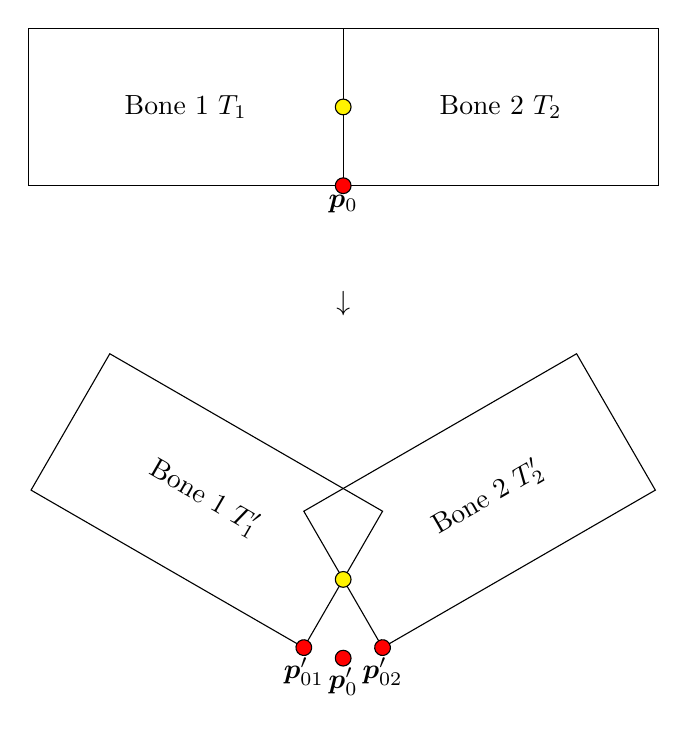
\begin{tikzpicture}
    \draw (0,0) rectangle (4,2);
    \draw (4,0) rectangle (8,2);
    \node at (2,1) {Bone 1 $T_1$};
    \node at (6,1) {Bone 2 $T_2$};
    \filldraw[draw=black,fill=red] (4,0) circle (.1) node[anchor=north]
    {$\bm p_0$};
    \filldraw[draw=black,fill=yellow] (4,1) circle (.1);

    \node at (4,-1.5) {$\downarrow$};

    \draw[rotate around={-30:(4,-5)}] (4,-6) rectangle (0,-4);
    \draw[rotate around={30:(4,-5)}] (4,-6) rectangle (8,-4);
    \node[rotate around={-30:(4,-5)}] at (-0.8,-5.3) {Bone 1 $T'_1$};
    \node[rotate around={30:(4,-5)}] at (7.8,-1.3) {Bone 2 $T'_2$};
    \filldraw[draw=black,fill=yellow] (4,-5) circle (.1);

    \filldraw[draw=black,fill=red,rotate around={-30:(4,-5)}] (4,-6)
        circle (.1) node[anchor=north] (A) {$\bm p'_{01}$};
    \filldraw[draw=black,fill=red,rotate around={30:(4,-5)}] (4,-6)
        circle (.1) node[anchor=north] (B) {$\bm p'_{02}$};
    \filldraw[draw=black,fill=red] (4,-6) circle(.1) node[anchor=north]
        (C) {$\bm p'_0$};
\end{tikzpicture}

Vertex $\bm p_0$ has weights $w_{01} = 0.5$ and $w_{02} = 0.5$. Points
$\bm p'_{01}$ and $\bm p'_{02}$ are generated by transforming point
$\bm p_0$ using $T'_1$ and $T'_2$. $\bm p'_0$ can be determined using
$\bm p'_0 = w_{01}\bm p'_{01} + w_{02}\bm p'_{02} = 0.5\bm p'_{01} + 0.5
\bm p'_{02}$.

\section{Raytracing}

\subsection{Geometry representation}

A ray is represented as $\bm p(t) = \bm o + \bm d t$, $\bm o$
being the ray origin and $\bm d$ being the ray direction. All
solutions for $t$ under section 2.1 refer
to the $t$ parameter for $\bm p(t)$.

\subsubsection{Sphere}

Implicit equation: $H(\bm P) = \bm P \cdot \bm P - r^2 = 0$

Intersection detection ($\bm c_o$ is origin, $\bm R_d$ is
normalized ray direction, $\bm c_s$ is sphere center, $r$ is
sphere radius)
\begin{gather*}
    \bm c_{\Delta} = \bm c_s - \bm c_o\\
    a = \bm R_d \cdot \bm R_d\\
    b = 2(\bm c_{\Delta} \cdot \bm R_d)\\
    c = \bm c_{\Delta} \cdot \bm c_{\Delta} - r^2\\
    d = b^2 - 4ac\\
    t = \frac{b \pm \sqrt{d}}{2a}
\end{gather*}

If $d < 0$, there is no intersection. If both solutions for $t$
are negative, there is no intersection.
If only one solution for $t$ is positive, that is where the
intersection occurs. If both solutions for $t$ are positive,
the intersection occurs at the closest $t$.

\subsubsection{Triangle}

Any point $\bm P$ on a triangle $(\bm a,\bm b,\bm c)$ can be represented as $\bm P(
\alpha,\beta,\gamma) = \alpha \bm a + \beta \bm b + \gamma \bm
c$, with $\alpha + \beta + \gamma = 1$.

\end{document}
